% !TEX encoding = UTF-8
% !TEX TS-program = pdflatex
% !TEX root = data mining.tex
% !TEX spellcheck = it-IT
\chapter{Lezione 3 - Modello lineare
semplice}\label{lezione-3---modello-lineare-semplice}

\begin{itemize}
\item
  \textbf{OLTP}: strumenti di interrogazione su specifiche informazioni
  da rihicedere ai vari database, detti operativi
\item
  \textbf{OLAP}: \ldots{}
\item
  \textbf{KDD}: Knowledge discovery database, si parte da uno o più
  database operativi per costruirne uno strategico, il data whare house;
  questa costruzione comporta anche un'operazione di omogeneizzazione di
  definizione di variabili e operazioni di pulizia dei dati (\textbf{data
  mining analitico}).
\end{itemize}

\section{Modelli}\label{modelli}

\textbf{Modello}: (o algoritmo) rappresentazione semplificata del
fenomeno di interesse, funzionale ad un obiettivo specifico.

Non esiste un modello vero in quanto si tratta di approssimazioni molto
dettagliate, ci sono dei modelli che in determinati contesti risultano
migliori di altri. Specialmente in ambiti non scientifici, il criterio
per la bontà di un modello è il \textbf{basta che funzioni}, questo
perché tipicamente i dati che vengono utilizzati non sono stati raccolti
con un criterio sperimentale.

Tipicamente il modello viene visto come una scatola nera, funziona ma
non si sa quale sia il vero meccanismo che regola il fenomeno. Tuttavia,
questa black box deve essere comunque manutenuta, non basta avere
solamente l'hardware e il software.

\subsection{Il modello lineare
semplice}\label{il-modello-lineare-semplice}

Si parte da due variabili e si costruisce un modello che li mette in
relazione tra loro.

Il data set di riferimento riguarda i dati di 200 mercati su cui opera
un'azienda, per i quali si conosce la quantità di merce venduta in
migliaia e il budget speso per la pubblicità radiofonica in quella
zona.

Si vuole ottenere un'equazione che permetta di prevedere le vendite in
funzione del budget.

Il primo passo è quello del costruire un grafico di dispersione, dove
nelle \emph{x} ci sono le spese e nelle \emph{y} ci sono le unità
vendute.

\begin{figure}[htbp]
\centering
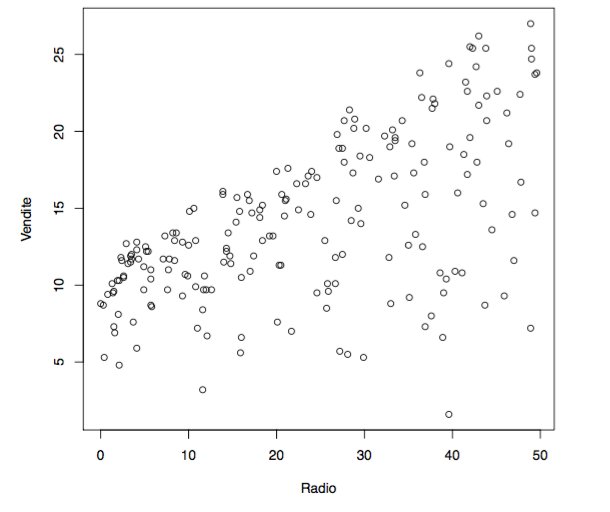
\includegraphics{./notes/immagini/l3-figura1.png}
\caption{Grafico di dispersione per il data set delle vendite}
\end{figure}

Dal grafico si può osservare un andamento lineare che può essere
approssimata con:

$$
vendite = \beta_0 + \beta_1 (radio) + (errore)
$$

dove la componente \emph{errore} esprime la parte delle vendite non
legate alle pubblicità via radio.

Un modello di questo tipo prende il nome di \textbf{modello di
regressione lineare semplice}.

La variabile \emph{y} (\emph{vendite}) prende il nome di
\textbf{variabile risposta/dipendente/output} mentre \emph{x}
(\emph{radio}) prende il nome di \textbf{variabile
esplicativa/indipendente/input} e i vari coefficiente \emph{beta}
prendono il nome di \textbf{parametri}.

Il gioco adesso diventa quello di andare a trovare dei valori
\emph{b\^{}0} e \emph{b\^{}1} che approssimano la retta nel miglior modo
possibile. La ricerca avviene utilizzando i dati presenti nel data set:


\begin{align*}
	y_1 &\approx \hat{\beta}_0 + \hat{\beta}_1 x_1 \\
	y_2 &\approx \hat{\beta}_0 + \hat{\beta}_1 x_2 \\
	&\ldots \\
	y_n &\approx \hat{\beta}_0 + \hat{\beta}_1 x_n
\end{align*}

Raffinando l'idea si ottiene il metodo dei \textbf{minimi quadrati}

$$
s^2(\beta_0, \beta_1) = \sum\limits_{i=1}^n(y_i - \beta_0 - \beta_1 x_i)^2
$$

e si vanno a cercare i parametri che minimizzano l'errore di stima
ai minimi quadrati.

$$ s^2(\hat{\beta}_0,\hat{\beta}_1) \leq s^2(\beta_0, \beta_1) $$

Si utilizza il quadrato della distanza, sia per rendere l'errore
indipendente dal segno, sia per dare maggior peso ad errori maggiori.

Ci sono un po' di barbatrucchi matematici per trovare il minimo quello
che interessa è:

\begin{align*}
	\beta_1 &= \frac{\sum\limits_{i=1}^{n} (x_i - \bar{x})(y_i - \bar{y})}{ \sum\limits_{i=1}^{n} (x_i - \bar{x})^2} \\
	 &= \frac{cov(X,Y)}{var(X)} \\
	 \: \\
	\beta_0 &= \bar{y} - \beta_1 \bar{x}
\end{align*}

Da notare che nel lato pratico non ci sarà mai un dataset con varianza
nulla, perché in quel caso il problema di regressione non ha senso. Per
il dataset delle vendite si ottiene come retta ai minimi quadrati

\begin{figure}[htbp]
\centering
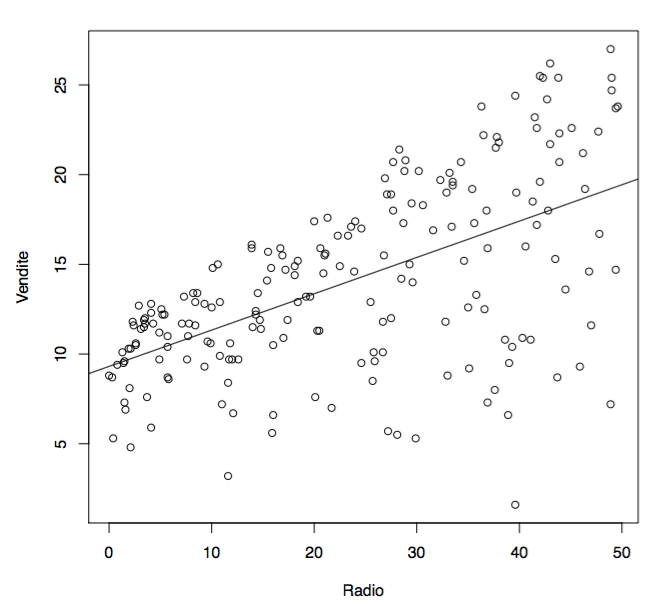
\includegraphics{./notes/immagini/l3-figura5.png}
\caption{Retta ai minimi quadrati per il dataset delle vendite}
\end{figure}

\subsubsection{Residui}\label{residui}

Non è detto che la retta approssimi bene i dati, anche se è quella dei
minimi quadrati.

Un indicatore dell'andamento è dato dai \textbf{residui}, che
rappresentano la differenza tra i valori osservati e quelli ottenuti
utilizzando la retta.

$$ r_i = y_i - \hat{\beta}_0 - \hat{\beta}_1x_i \: \: \forall i = 1, \ldots, n$$

Per costruzione della retta, la somma di tutti i residui risulta essere
0, quindi, per valutare la retta è necessario utilizzare la
\textbf{varianza} dei residui. Minore è la varianza, migliore è la
retta.

Nel caso peggiore, la varianza dei residui ha come bound superiore la
varianza della risposta, ovvero \emph{var(Y)}.

È quindi possibile definire il \textbf{coefficiente di determinazione}:

$$
R^2 = 1 - \frac{var(r_i, \ldots, r_n)}{var(Y)}
$$

$R^2$ varia tra 0 e 1, dove 1 è il valore ottimo e 0 è il valore
peggiore.

Da notare che ciò vale solo per la retta.
